\section{Terminal}
Aujourd'hui, tous les ordinateurs ont une interface graphique, qu'on pilote principalement avec la souris; le clavier ne sert plus qu'à taper du texte. Cependant, il n'en a pas toujours été ainsi! Au début de l'informatique, toutes les interactions se faisaient au clavier, dans ce qu'on appelle la \textbf{console}, ou \textbf{terminal} (figure \ref{terminal}).

\begin{figure}[h!]
\begin{center}
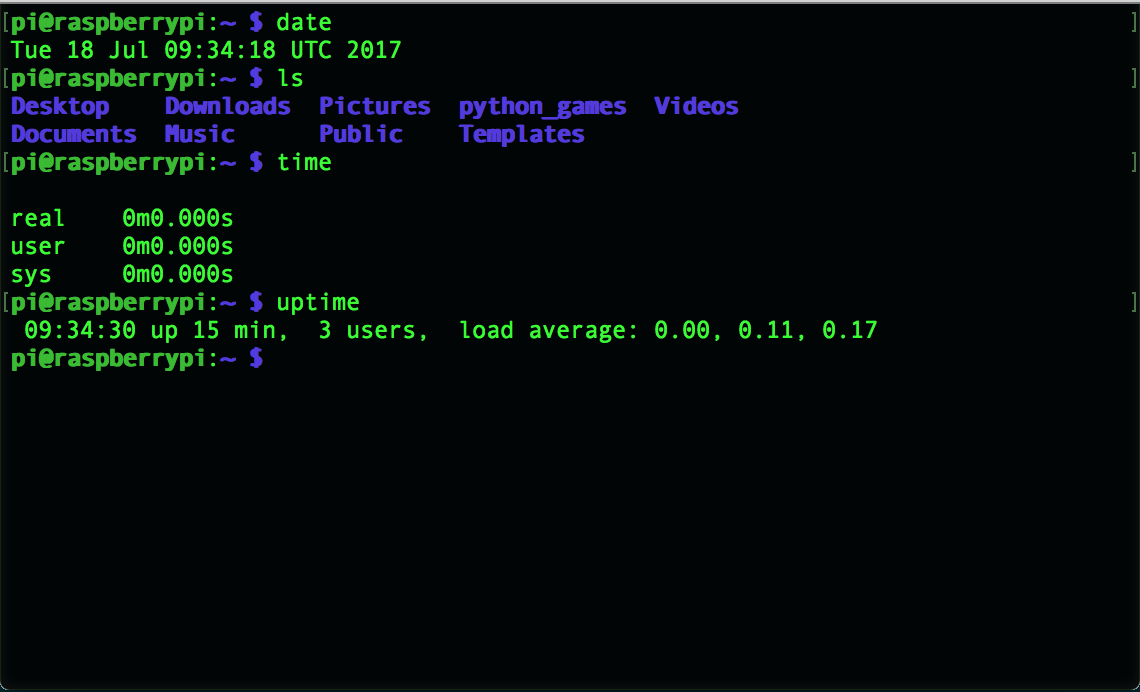
\includegraphics[width=10cm]{img/ssh.png}
\end{center}
\caption{Le terminal}
\label{terminal}
\end{figure}

Bien que sur Windows ou macOS, on n'utilise presque plus le terminal, il a encore une certaine utilité sur les distributions Linux, dont Raspbian fait partie.
Il existe des commandes très pratiques pour rapidement mettre à jour ses programmes, ou bien configurer certains aspects du Raspberry Pi.

On accède au terminal du Raspberry Pi en appuyant sur la quatrième icône de la barre des menus (voir figure \ref{interface}) ou en appuyant simultanément sur \textit{CTRL + ALT + T}.

\section{Accéder au Raspberry Pi}
Il existe de nombreuses manières d'accéder au Raspberry Pi. Nous détaillerons ici les principales.

\begin{figure}[h!]
    \begin{center}
        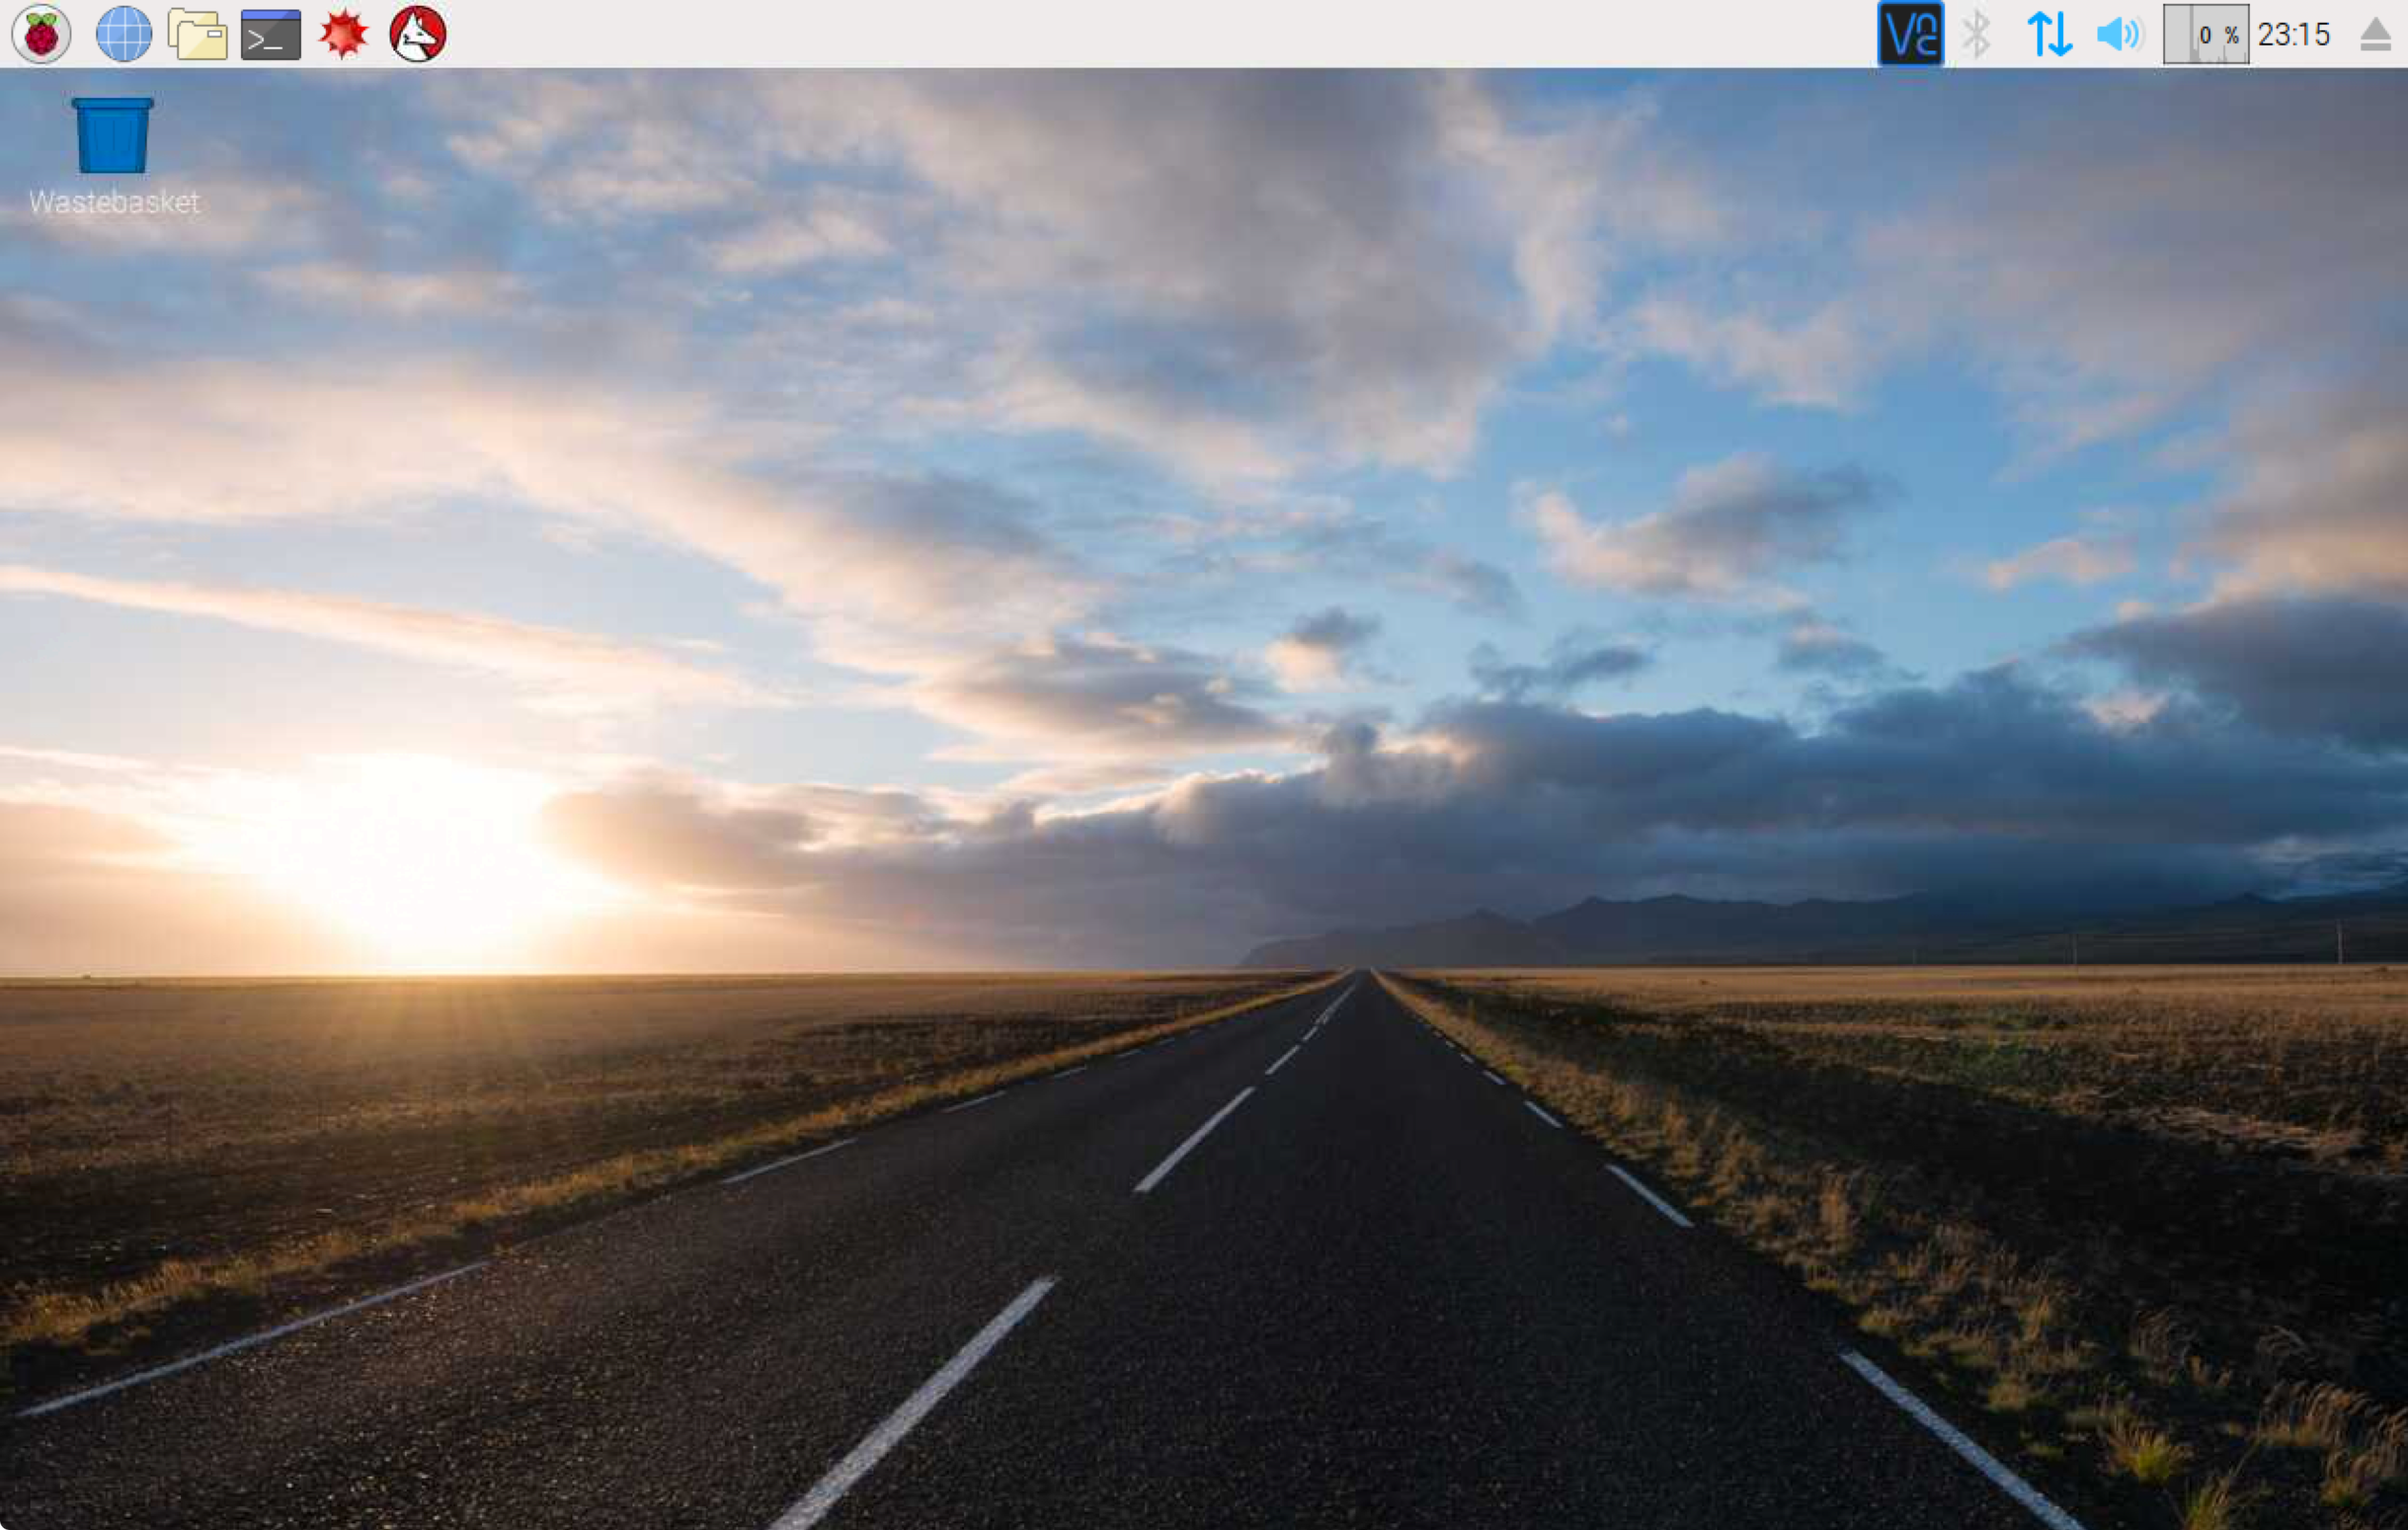
\includegraphics[width=15cm]{img/raspi.png}
    \end{center}
    \caption{Interface graphique du Raspberry Pi}
    \label{interface}
\end{figure}

\subsection{Connexion directe}

La plus simple est bien sûr de se connecter à un écran via le port HDMI. La connexion est directe, et très fiable. Cependant, on n'a pas toujours un écran libre à disposition, et c'est là que les techniques de connexion suivantes pourront montrer leurs avantages.

\subsection{Connexion SSH (\textit{Secure Shell})}

Il s'agit ici de se connecter au terminal du Raspberry Pi. On n'aura pas accès à l'interface graphique, ce qui complique certaines opérations. Cependant, pour lancer un script ou mettre à jour quelques programmes, c'est un moyen rapide d'accéder au Raspberry Pi.

On se connecte au terminal du Raspberry Pi... par le terminal d'un autre ordinateur! Sur Windows, le programme s'appelle Console, sur macOS simplement Terminal. Une fois le programme ouvert, on trouve d'habitude une simple ligne de texte, et beaucoup d'espace dans lequel écrire des commandes.

Voici celle qui nous permet de nous connecter :

\texttt{ssh nom\_utilisateur@serveur}

Quand on configure le Raspberry Pi, un nom d'utilisateur par défaut est créé, il s'agit simplement de \texttt{pi}. Quant au serveur, ce peut-être une URL (une adresse, comme \texttt{raspberry.serveur.com} par exemple), ou bien une adresse IP (plus compliqué, il existe plusieurs types, mais on retiendra qu'il s'agit d'une suite de chiffres séparés par des points, comme ceci par exemple : \texttt{192.168.1.314}).

Nous vous aiderons à trouver l'adresse du serveur.

Une fois qu'on a l'adresse du serveur, on entre la commande, et un mot de passe est demandé. A nouveau, le Raspberry Pi en a un par défaut : \texttt{raspberry}.

On entre le mot de passe (il ne s'affiche pas, c'est tout-à-fait normal, il faut le taper à l'aveugle), et on a enfin accès au terminal du Raspberry Pi! Pour voir si tout fonctionne, essayez de taper la commande \texttt{uptime}. C'est le temps qu'est resté allumé votre Raspberry Pi depuis qu'on l'a branché à l'alimentation!

\subsection{Connexion VNC}

Ce type de connexion à distance est beaucoup plus agréable : on accède à l'interface graphique, mais via Internet, et non plus via un câble. Ce qui veut dire que si votre appareil est branché à Internet, vous pouvez potentiellement y accéder depuis n'importe où dans le monde!

Pour activer VNC sur le Raspberry Pi, il faut aller dans le terminal, et taper la commande \texttt{sudo raspi-config}. Puis sur l'interface qui s'affiche, on descend avec les flèches du clavier jusqu'à \texttt{Interfacing Options}. On valide avec la touche Entrée. L'option \texttt{VNC} apparaît, il suffit de l'activer.

On va aussi modifier la résolution tant qu'on y est. Il faut cette fois se rendre sur \texttt{Advanced Options} $\rightarrow$ \texttt{Resolution}. Une résolution de 1280x1024 devrait suffire!

\begin{figure}[h!]
    \begin{center}
        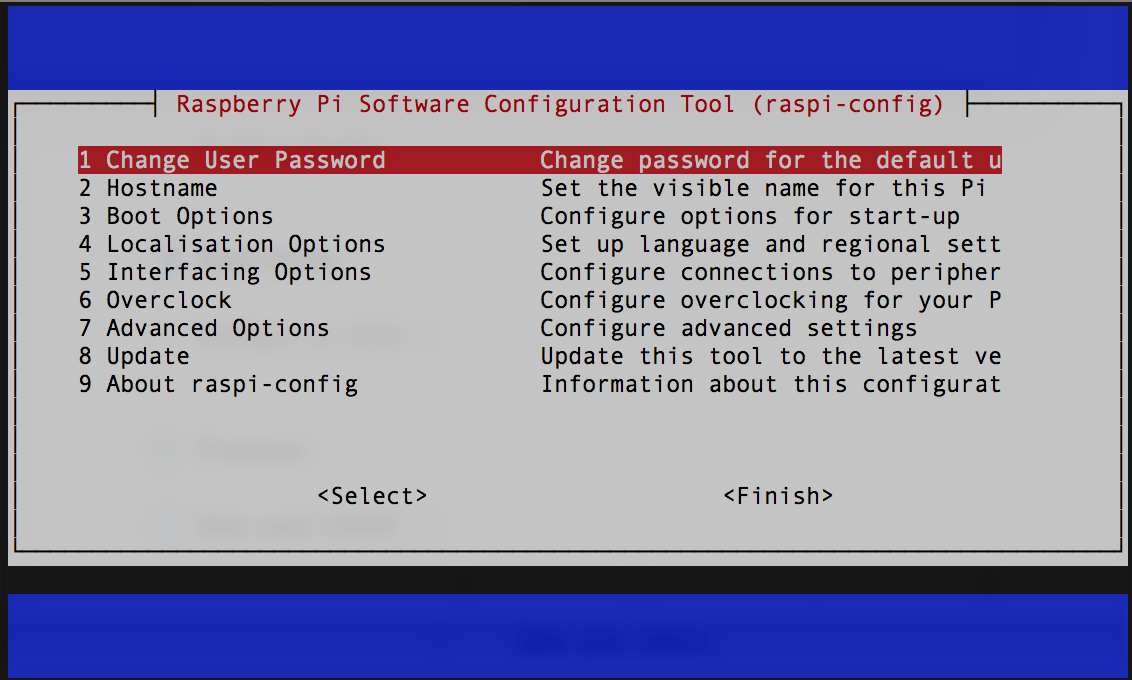
\includegraphics[width=8cm]{img/raspi-config.png}
    \end{center}
    \caption{raspi-config}
    \label{raspi-config}
\end{figure}

C'est tout pour la configuration sur le Raspberry Pi! A partir de maintenant, plus besoin d'y toucher. Sur notre autre ordinateur maintenant, il faut télécharger un client VNC : \url{https://www.realvnc.com/en/download/vnc/}.

En lançant le programme VNC Connect, il nous est demandé l'adresse du serveur VNC. C'est la même que pour le serveur qu'on a du indiquer lors de la connexion SSH. Ensuite, une fenêtre s'ouvre pour demander l'utilisateur et le mot de passe. Rappelez-vous : par défaut, il s'agit respectivement de \texttt{pi} et \texttt{raspberry}.

\section{Mettre à jour son Raspberry Pi}
Raspbian possède une fonction très pratique : on peut mettre à jour tous ses programmes, en même temps et avec seulement deux commandes très pratiques!

Tapez simplement successivement dans le terminal (via SSH ou via l'interface graphique du Raspberry Pi)/

\texttt{sudo apt-get update}

\texttt{sudo apt-get upgrade}

Il est possible qu'une confirmation soit demandée : tapez simplement \texttt{yes} ou \texttt{Y}, selon les cas.
Après quelques téléchargements et installations diverses, c'est fini : tout l'appareil est à jour! Facile, non?

\section{Installer Python 3}
Par défaut, le Raspberry Pi n'est plus livré avec Python 3. Heureusement, c'est facile à installer! Tapez simplement la ligne suivantes dans le terminal :\\

\texttt{sudo apt-get install python3}\\


\section{Utilisation Python sur Raspberry}

Pour lancer un code python sur le raspberry, plus besoin d'installer un programme supplémentaire. Il est possible d'écrire le code grâce à n'importe quel éditeur de texte tel que "text editor" ou "atom" et lancer le code directement via le terminal (toujours bien utile celui-là) en tapant la commande suivante : \\

\texttt{python3 nom\_du\_script.py}\\


\section{Mini-jeu}
Exercice à réaliser en cours.

\section{Radar de recul}
Le Raspberry PI est un ordinateur embarqué, il permet donc de réaliser des systèmes utilisant des capteurs et pouvant interagir avec son environnement. Pour ce projet final, vous disposez d'un capteur à ultrasons permettant de mesurer une distance. Nous allons donc l'utiliser pour réaliser un radar de recul comme ceux présent dans les voiture, nous avertissant de l'approche d'un objet.

L'utilisation de ce capteur ne nécessite aucune installation mais pour faciliter un peu les choses, voici un script Python permettant de mesurer la distance :

\begin{python}
import RPi.GPIO as GPIO
import time

GPIO.setmode(GPIO.BCM)

GPIO_TRIGGER = 18   # PIN connecte a la borne TRIGGER du capteur
GPIO_ECHO = 24      # PIN connecte a la borne ECHO du capteur

GPIO.setup(GPIO_TRIGGER, GPIO.OUT)
GPIO.setup(GPIO_ECHO, GPIO.IN)

def distance():
    # set Trigger to HIGH
    GPIO.output(GPIO_TRIGGER, True)

    # set Trigger after 0.01ms to LOW
    time.sleep(0.00001)
    GPIO.output(GPIO_TRIGGER, False)

    StartTime = time.time()
    StopTime = time.time()

    # save StartTime
    while GPIO.input(GPIO_ECHO) == 0:
        StartTime = time.time()

    # save time of arrival
    while GPIO.input(GPIO_ECHO) == 1:
        StopTime = time.time()

    # time difference between start and arrival
    TimeElapsed = StopTime - StartTime
    # multiply with the sonic speed (34300 cm/s)
    # and divide by 2, because there and back
    distance = (TimeElapsed * 34300) / 2

    return distance

def cleanup():
    GPIO.cleanup()

\end{python}

Cette fonction permet de lire la distance mesurée par le capteur. En appliquant toutes les notions vues lors de la semaine, réalisez un programme qui allume les LED en fonction de la distance.
